% =====================================================================
%  DESARROLLO  —  una sección por objetivo específico, que es como
%  REQUISITOS.md rastrea el trabajo (matriz RF <-> OE <-> prueba).
% =====================================================================
\chapter{Desarrollo}

El sistema se construyó en cuatro frentes, uno por objetivo específico. Cada
sección describe qué se hizo, qué decisión se tomó y por qué. Las decisiones que
hubo que revisar aparecen con su corrección, porque el camino que se descartó
explica el que quedó.

% ---------------------------------------------------------------------
\section{Arquitectura funcional del sistema (OE1)}

La figura~\ref{fig:arquitectura} resume el sistema completo. Están la interfaz
por la que entra la solicitud, el coordinador que la reparte, los dos agentes con
su pila de navegación y la zona de transición donde ocurre el relevo. El
protocolo de la parte inferior es la secuencia que el §3.1.2 implementa.

\begin{figure}[H]
  \centering
  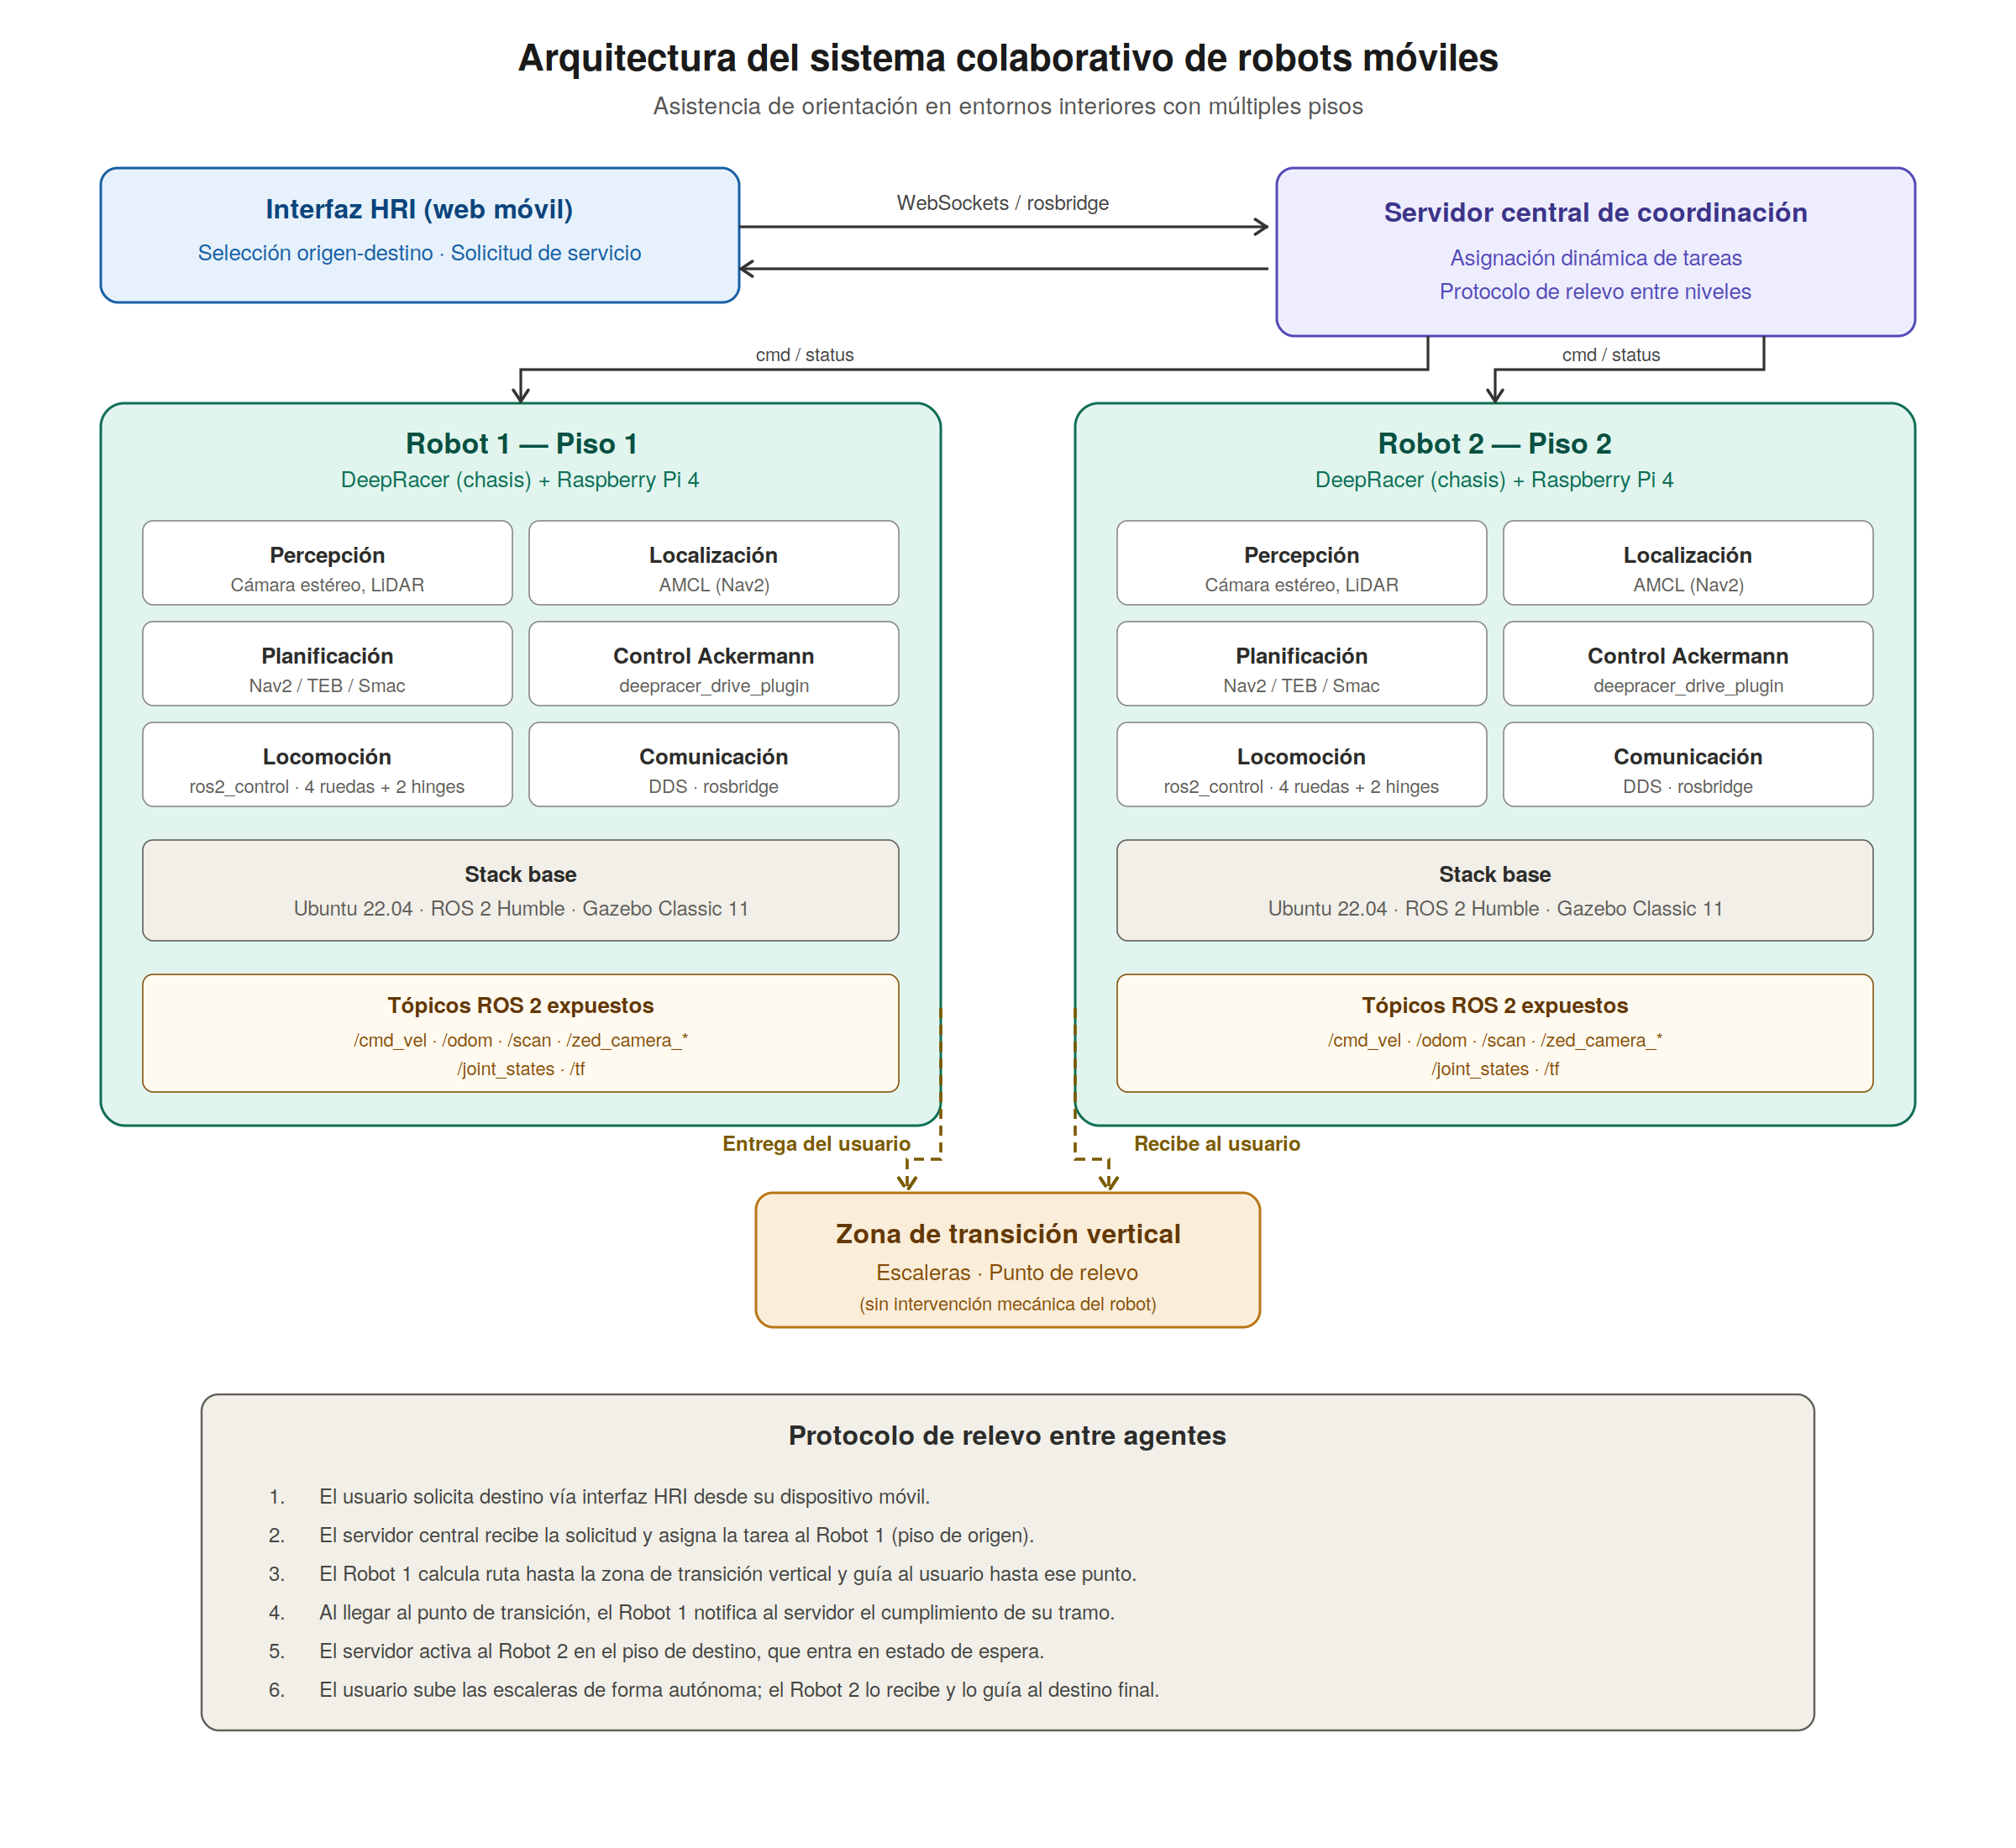
\includegraphics[width=\textwidth]{imagenes/arquitectura_sistema.png}
  \caption{Arquitectura funcional del sistema colaborativo, tal como quedó
    modelada en el OE1. Ningún robot atraviesa la zona de transición: lo que la
    cruza es el usuario, y lo que se traspasa entre agentes es la
    responsabilidad de guiarlo.}
  \label{fig:arquitectura}
\end{figure}

Dos casillas de la figura se concretaron más tarde, y conviene decirlo para que
el lector no las lea como definitivas. La de planificación nombra los candidatos
que se consideraron en el diseño; cuál quedó y por qué está en el §3.2.3. Y los
niveles aparecen como pisos 1 y 2 porque así se planteó el escenario. Al cambiar
de sitio de pruebas pasaron a ser los pisos 3 y 4 (§3.2.5), y la arquitectura no
cambió. Que no cambiara es justamente lo que se esperaba de ella.

\subsection{El contrato de interfaces}

Antes de escribir código se fijó un contrato: qué habla con qué y en qué formato.
El sistema tiene tres piezas. Un \textbf{coordinador} central decide y manda. Dos
\textbf{agentes}, uno por nivel, ejecutan. Y una \textbf{interfaz web} por la que
el usuario pide el servicio.

La comunicación sigue tres reglas que no se rompen:

\begin{enumerate}[leftmargin=*]
  \item El coordinador manda a un agente \textbf{solo} mediante la acción de
    navegación de ROS~2. No publica velocidades directamente.
  \item La interfaz habla \textbf{solo} con el coordinador. Nunca con los
    agentes.
  \item El texto que ve el usuario lo redacta el coordinador. La interfaz lo
    muestra literal.
\end{enumerate}

La tercera evita que la lógica de presentación se duplique en el navegador. Si el
cliente interpretara el estado numérico para decidir qué mostrar, habría dos
copias de la misma lógica y acabarían divergiendo.

\subsection{El planificador, escrito sin ROS a propósito}

El relevo es el aporte declarado del proyecto. Por eso se escribió como función
pura: entran el catálogo de puntos y un par origen-destino, salen los tramos que
hay que ejecutar. No importa el middleware ni mantiene estado.

La razón es de verificabilidad. Si el relevo viviera dentro del nodo, mezclado
con clientes de acción, la única forma de comprobarlo sería levantar dos
simuladores y mirar si el carro llega. Eso es lento y frágil. Como función pura
se agota en milisegundos: \textbf{la prueba recorre 930 combinaciones de
origen-destino y verifica cada plan, sin simulador}.

Esa prueba encontró defectos que una corrida no habría delatado. El más claro:
cuando el origen o el destino \emph{es} el punto de transferencia de su nivel, el
plan mandaba al mismo robot dos veces a la misma pose. Un desplazamiento de cero
metros no falla en Nav2 —devuelve éxito al instante— así que la simulación no lo
habría mostrado.

\subsection{La asignación de tareas}

Cada nivel tiene un robot asignado, y esa correspondencia es un dato de
configuración, no una constante del código. El coordinador elige el agente al
aceptar la solicitud, según el nivel del origen y del destino.

En la taxonomía de \textcite{gerkey2004taxonomy} es una asignación
centralizada e instantánea. Con dos agentes y el nivel decidiendo cuál responde,
un esquema de subasta añadiría complejidad sin dar flexibilidad.

El planificador exige \textbf{exactamente un punto de transferencia por nivel} y
falla con un mensaje explícito si encuentra dos. Hoy cada planta tiene una
escalera y eso se cumple. La verificación está puesta para que el día que haya
dos la decisión se tome a la vista, y no en silencio.

% ---------------------------------------------------------------------
\section{Plataforma robótica (OE2)}

\subsection{Por qué DeepRacer y no DonkeyCar}

El OE2 habla de «dos vehículos tipo DonkeyCar». Los vehículos empleados son dos
AWS DeepRacer, y el cambio conviene explicarlo porque el lector lo va a notar.

DonkeyCar y DeepRacer son la misma clase de plataforma: un chasis de
radiocontrol a escala 1:18 con dirección Ackermann, un computador a bordo y
software abierto. Lo que el objetivo fija —cinemática tipo automóvil, bajo costo,
código modificable— se cumple igual con una que con otra. La diferencia es que la
universidad ya tenía los dos DeepRacer, de modo que usarlos evitó construir
hardware y dejó ese tiempo para el problema que el proyecto declara como suyo,
que es la coordinación.

El cambio no sale gratis y hay que decirlo. El DeepRacer trae su propia pila de
software, pensada para conducción autónoma por visión y para competencia, y buena
parte del trabajo del §3.2.3 consistió en convivir con ella. Un DonkeyCar partiría
de menos capas, pero habría que montarlo.

\subsection{Nav2 sobre un vehículo que no gira sobre su eje}

La plataforma sigue cinemática tipo automóvil. No es holonómica: no puede girar
en el sitio. La configuración por omisión del marco de navegación de ROS~2 asume
tracción diferencial, de modo que propone trayectorias que el vehículo no puede
ejecutar.

Se sustituyeron dos de sus tres capas. La planificación global pasó a un
planificador híbrido A* con modelo Reeds-Shepp, que admite marcha atrás y genera
las maniobras de inversión que el vehículo necesita. El control de seguimiento
pasó a un controlador de persecución pura regulada, con marcha atrás habilitada.
Del árbol de comportamiento se quitó la recuperación que gira sobre el propio
eje, porque el vehículo no puede hacerla.

\subsection{El orden de puesta en marcha}

Cada pieza de la cadena de navegación solo se puede diagnosticar si la anterior
funciona. La guía oficial de puesta en marcha de Nav2 \autocite{nav2setup} lo
plantea como una escalera de siete peldaños. De abajo arriba: transformaciones
entre marcos, odometría, barrido del láser, mapa, localización, mapas de costos
y, al final, planificador y controlador.

El proyecto la siguió en ese orden, y fue lo que permitió aislar el fallo del
apartado siguiente. Sin la escalera, una odometría que no mide se confunde con un
planificador que no planifica, porque los dos se manifiestan igual: el vehículo no
llega. Con ella, el problema queda acotado a un peldaño.

El orden importa además en la ejecución. Los mapas de costos leen el mapa al
configurarse. Si el servidor de mapas no está activo en ese instante, la capa
estática queda vacía. Y entonces el planificador rechaza cualquier meta diciendo
que el punto de partida está ocupado. El mensaje señala el origen, y la causa está tres
peldaños más abajo.

\subsection{La odometría, que fue el cuello de botella}

El vehículo no tiene encoders de rueda. Su única fuente de odometría es la
correspondencia entre barridos sucesivos del láser. Durante meses esa pieza no
funcionó, y el proyecto tardó en entender por qué.

La causa no era de calibración sino de información. En un pasillo recto y de
sección uniforme, cada barrido es prácticamente idéntico al anterior a lo largo
del eje del corredor. El estimador devuelve un desplazamiento cercano a cero y
\emph{acierta}: desde el sensor no ha cambiado nada. Se midió sobre el edificio y
el resultado fue contundente: en los pasillos disponibles la odometría registraba
entre el 5~\% y el 73~\% del avance real.

La figura~\ref{fig:hall} muestra lo que eso produce. Las tres trayectorias son
del mismo vehículo en el mismo hall. La localización se desplaza hasta más de dos
metros respecto de donde el vehículo estaba de verdad, medido con flexómetro, y
en una de las corridas salta fuera del recinto. La línea a trazos marca otro
hallazgo de esa misma sesión: la pared norte estaba modelada 0,84~m más al norte
de lo que está.

\begin{figure}[H]
  \centering
  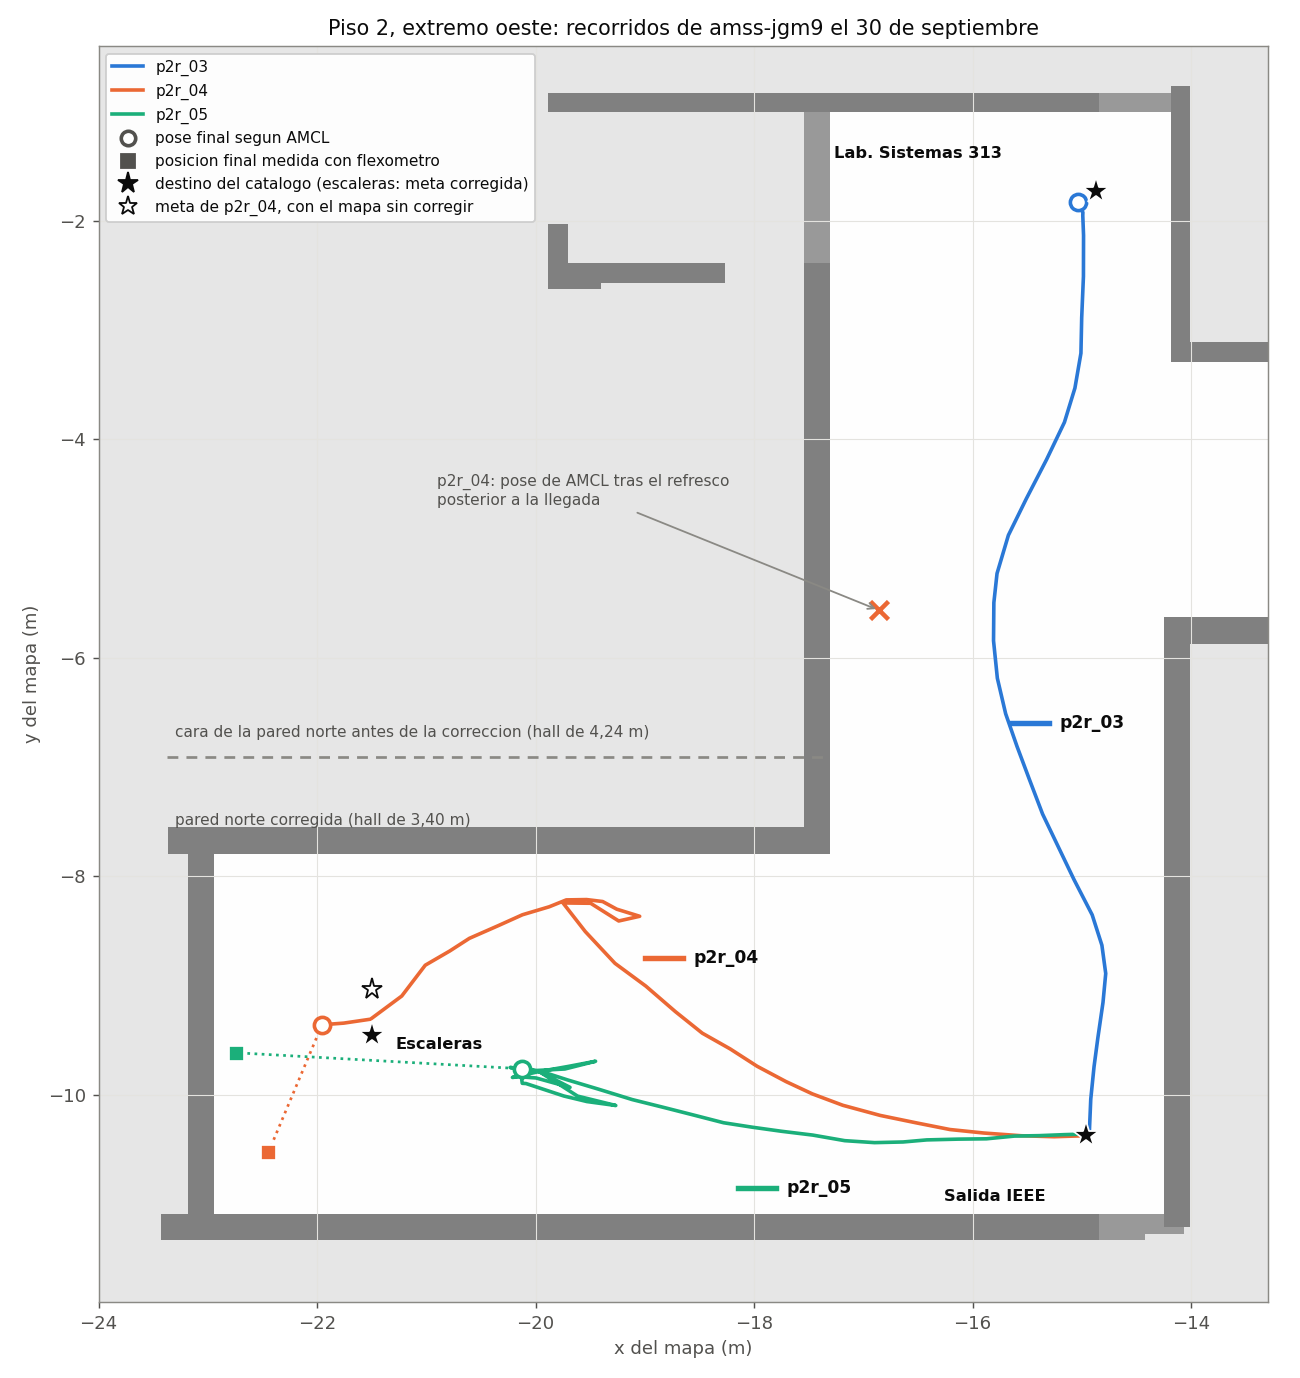
\includegraphics[width=0.78\textwidth]{imagenes/recorridos_hall_piso2.png}
  \caption{Tres recorridos en el hall del piso 2. El círculo es la pose que
    reporta la localización al terminar; el cuadrado, la posición real medida con
    flexómetro. La separación entre los dos es el error, y su causa está en la
    odometría, no en el algoritmo de localización.}
  \label{fig:hall}
\end{figure}

La solución no fue afinar el algoritmo, porque no había nada que afinar. Fue
cambiar de entorno. El criterio para elegirlo salió de la misma medida: hace
falta estructura no uniforme dentro del alcance del sensor durante todo el
recorrido.

Se levantaron con flexómetro dos plantas que la tienen. Entre las tres hornacinas
de salón, los lockers, la papelera, el ascensor y la escalera suman ocho cambios
de perfil en 25~m, uno cada tres metros. Con la misma odometría y sin tocar un
parámetro, el error cayó a menos del 5~\%.

\subsection{Los mapas, derivados de medidas y no de SLAM}

El proyecto intentó durante semanas construir el mapa con SLAM y no lo consiguió
en ningún pasillo, por la misma razón del apartado anterior. La vía que
funcionó fue otra: \textbf{levantar la planta con flexómetro y derivar de ese
levantamiento tanto el mundo simulado como el mapa de navegación}.

Eso tiene una consecuencia que conviene subrayar. Simulación y edificio coinciden
porque salen de la misma fuente, no porque se parezcan. El proyecto había dado
esa correspondencia por supuesta, y al verificarla por primera vez resultó falsa:
el modelo anterior daba un hall 0,84~m más ancho de lo que es, un 20~\% de error.

La herramienta que genera las plantas incluye una comprobación que no se salta.
Un pasillo mide lo mismo por sus dos lados, así que suma las dos paredes y avisa
si no cierran dentro del 2~\%. Esa comprobación encontró cinco errores antes de
generar nada. Las dos plantas cierran al 0,32~\% y al 0,62~\%.

La figura~\ref{fig:mapa4} es el resultado para una de ellas. Lo que se ve no es
un plano dibujado sino el mapa de ocupación con el que navega el vehículo,
generado a partir de las medidas. Los entrantes de los salones, los lockers, el
ascensor y la escalera son los ocho cambios de perfil que hacen observable el
avance.

\begin{figure}[H]
  \centering
  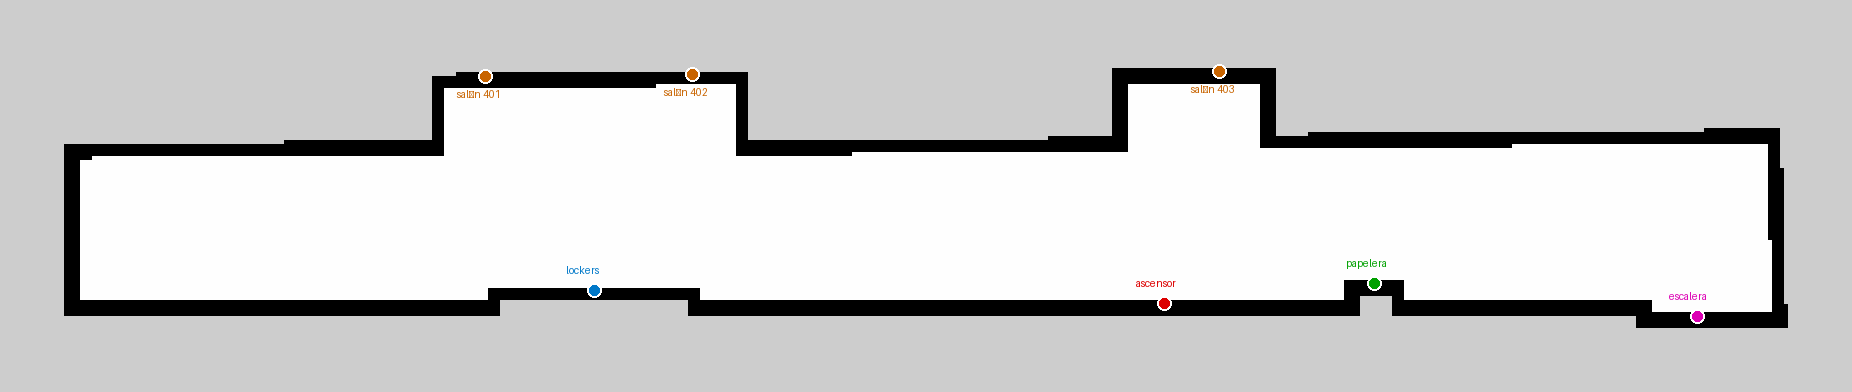
\includegraphics[width=\textwidth]{imagenes/mapa_piso4.png}
  \caption{Mapa de navegación del piso 4, derivado del levantamiento con
    flexómetro. El pasillo corre 25~m del extremo norte al sur; los salones
    quedan al este, y el ascensor y la escalera al oeste.}
  \label{fig:mapa4}
\end{figure}

\subsection{La banda muerta de tracción, y lo que obliga a configurar}

Al integrar la cadena de tracción apareció una característica de la plataforma
que condiciona toda la aproximación al destino. \textbf{El vehículo no se mueve
con velocidad comandada por debajo de 0,40~m/s.} El puente que traduce la orden
de velocidad a la señal del variador la convierte en tracción nula, y lo hace sin
emitir ningún aviso: desde fuera parece que la orden se ejecutó.

Eso forzó una decisión de configuración que conviene dejar escrita, porque tiene
consecuencias. La velocidad mínima de aproximación del controlador se subió a ese
mismo valor, 0,40~m/s. Sin ese ajuste el vehículo se detenía al entrar en la fase
final del recorrido y se quedaba ahí, intentando moverse a una velocidad que su
propia cadena anulaba.

El efecto es que \textbf{el vehículo se aproxima a la meta a 0,40~m/s y no puede
ir más despacio}. No tiene régimen de aproximación fina. Es un límite de la
plataforma, no del software, y no se corrige afinando el controlador: las dos
salidas son bajar el umbral de arranque del vehículo —por mecánica o por
calibración de los servos— o fijar la tolerancia de llegada en un valor
compatible con la plataforma, con justificación previa. Las dos son decisiones,
no ajustes, y por eso quedan planteadas en el capítulo de trabajos futuros.

% ---------------------------------------------------------------------
\section{Interfaz humano-robot (OE3)}

\subsection{Una página web, no una aplicación}

El OE3 pide «una interfaz móvil». Lo que se construyó es una página web que se
abre en el navegador del teléfono. Cumple el objetivo: es móvil porque se usa
desde el teléfono del usuario. Y lo cumple mejor que una aplicación nativa. Un
visitante ocasional —que es el usuario que el proyecto declara— no va a instalar
nada para preguntar por un salón.

El requisito pedía que el usuario no instalara nada. La interfaz es una página
web que se abre desde el navegador del teléfono. No usa recursos externos,
porque debe funcionar sin salida a internet: en la red del edificio puede no
haberla.

La comunicación con el middleware pasa por un puente que expone las acciones de
ROS~2 como JSON sobre WebSocket. La librería de cliente más difundida del
ecosistema no servía: su cliente de acciones corresponde a la generación anterior
del middleware y es incompatible. La interfaz usa por eso un cliente propio,
escrito directamente sobre el protocolo del puente.

\subsection{Lo que el usuario ve}

El usuario elige origen y destino de un catálogo con búsqueda por nombre, y pulsa
un botón. A partir de ahí la página muestra el estado de la misión con el texto
que redacta el coordinador.

Dos funciones se añadieron después de ver el sistema en uso:

\textbf{Confirmación de cambio de piso.} La secuencia de una misión entre niveles
termina la etapa de transferencia cuando el robot del piso de destino llega a su
escalera. Pero el robot no puede saber si \emph{la persona} ya subió. Sin una
pausa explícita, la misión podía declararse completada con el usuario todavía en
el piso equivocado, y la instrumentación lo habría registrado como éxito.

\textbf{Cancelación.} El botón existía pero no hacía nada, y nadie lo había
notado: el servidor de acción no registraba la función de cancelación, de modo
que el middleware rechazaba toda solicitud por omisión y en silencio. Al
corregirlo se añadió además el comportamiento que faltaba: al cancelar, el robot
en curso regresa a su escalera antes de que la misión cierre.

% ---------------------------------------------------------------------
\section{Protocolo experimental (OE4)}

El protocolo se escribió \textbf{antes} de instrumentar el sistema, y esa
secuencia es deliberada. Fija las cuatro métricas con definición operativa, el
criterio de éxito, el tamaño de muestra y una lista cerrada de causas de
descarte con su techo.

Dos decisiones del protocolo merecen mención porque condicionan cómo se leen los
resultados.

La primera: \textbf{el éxito se mide contra la odometría del vehículo, nunca
contra el resultado que devuelve Nav2}. Una navegación puede terminar en
\emph{éxito} y haber dejado al robot lejos del destino. Aceptar ese resultado
sería dejar que el sistema se evalúe a sí mismo.

La segunda: \textbf{las misiones se sortean}. Con pares elegidos a mano se corre
el riesgo de probar justo los recorridos que funcionan.

Durante la escritura del analizador apareció un defecto que ninguna corrida
habría revelado, y que se trata en el §\ref{sec:limitaciones}: uno de los
criterios estaba formulado de manera que no podía dar resultado negativo.
